\documentclass[fontsize=12pt,paper=a4,twoside=semi,parskip=half-,headsepline,headinclude]{scrreprt}
% Grundgröße 12pt, zweiseitig
\usepackage[headsepline,automark]{scrlayer-scrpage}
% Seitenköpfe automatisch 
\usepackage[ngerman]{babel}
% Sprachpaket für Deutsch (Umlaute, Trennung,deutsche Überschriften)
\usepackage{blindtext}
% macht nur den Blindtext, den Sie aktuell sehen
\usepackage{lmodern}
% schöne PDF-Schrift
\usepackage{graphicx,hyperref,amssymb}
%Graphikeinbindung, Hyperref (alles klickbar, Bookmarks),
%Math. Symbole aus AmsTeX
\usepackage[utf8]{inputenc}
% Umlaute und über Tastatur einzugeben
\usepackage{listings}
\usepackage{xcolor}
% nette Listing-Formatierung
%\usepackage[backend=bibtex]{biblatex}
\usepackage[sorting=none, style=nature]{biblatex}
\addbibresource{literatur.bib}

% Festlegung Kopf- und Fußzeile     
\defpagestyle{meinstil}{%
{\headmark \hfill}
{\hfill \headmark}
{\hfill \headmark\hfill }
(\textwidth,.4pt)
}{%
(\textwidth,.4pt)
{\pagemark\hfill Philipp Ermer}
{\today \hfill \pagemark}
{\today\hfill\pagemark} 
}
\pagestyle{meinstil} 

\raggedbottom
\renewcommand{\topfraction}{1}
\renewcommand{\bottomfraction}{1}
\newcommand{\code}[1]{\texttt{#1}}

%%%%%%%%%%%%%%%%%%%%%%%%%%%%%%%%%%%%%%%%%%%%%%%%%%%%%%%%%%%%%%%%%%%%%%%%%%

\definecolor{dkgreen}{rgb}{0,0.6,0}
\definecolor{gray}{rgb}{0.5,0.5,0.5}
\definecolor{mauve}{rgb}{0.58,0,0.82}
\definecolor{blue}{rgb}{0,0,1}

\lstdefinelanguage{Kotlin}{
	keywords={package, import, as, typealias, class, interface, this, super, val, var, fun, for, null, true, false, is, in, throw, return, break, continue, object, if, else, while, do, try, when, companion, override, init, constructor, by, catch, finally, where, enum, sealed, annotation, data, inner, tailrec, operator, inline, infix, external, suspend, lateinit, vararg, reified, dynamic, public, private, protected, internal, out},
	keywordstyle=\color{blue},
	ndkeywords={@file, @property, @field, @get, @set, @receiver, @param, @setparam, @delegate, file, field, property, get, set, receiver, param, setparam, delegate, import, where},
	ndkeywordstyle=\color{blue},
	identifierstyle=\color{black},
	sensitive=true,
	comment=[l]{//},
	morecomment=[s]{/*}{*/},
	commentstyle=\color{dkgreen}\ttfamily,
	stringstyle=\color{mauve}\ttfamily,
	morestring=[b]",
	morestring=[b]',
}

\lstset{
	frame=tb,
	language=Java,
	aboveskip=3mm,
	belowskip=3mm,
	showstringspaces=false,
	columns=flexible,
	basicstyle={\small\ttfamily},
	numbers=none,
	numberstyle=\tiny\color{gray},
	keywordstyle=\color{blue},
	commentstyle=\color{dkgreen},
	stringstyle=\color{mauve},
	breaklines=true,
	breakatwhitespace=true,
	tabsize=3,
	morekeywords={var, out} % Hier wurden var und out hinzugefügt
}

	\DeclareUnicodeCharacter{03BB}{$\lambda$}
\begin{document}    % hier gehts los
	\renewcommand{\figurename}{Abb.}
	
  \thispagestyle{empty} % Titelseite

\includegraphics[width=0.2\textwidth]{hsh_icons/Wortmarke_WI_schwarz}

   {  ~ \sffamily
  \vfill
  {\Huge\bfseries Performance-Vergleich von \\Nebenläufigkeits-Konzepten in \\objektorientierten Programmiersprachen}
  \bigskip

  {\Large 
  Philipp Ermer \\[2ex]
 Master-Arbeit im Studiengang "`Angewandte Informatik"' 
 \\[5ex]
   \today } 
}
 \vfill
  
  ~ \hfill
  
\includegraphics[height=0.3\paperheight]{hsh_icons/H_WI_Pantone1665} 

\vspace*{-3cm}


\newpage 
\thispagestyle{empty}
\quad 


  \newpage \thispagestyle{empty}
 \begin{tabular}{ll}
{\bfseries\sffamily Autor} &  Philipp Ermer \\ 
            & Matrikelnummer: 1313395 \\
            & philipp.ermer@web.de \\[5ex]
{\bfseries\sffamily Erstprüfer:} & Prof. Dr. Holger Peine \\
          & Abteilung Informatik, Fakultät IV \\
         & Hochschule Hannover \\
        & holger.peine@hs-hannover.de \\[5ex]
{\bfseries\sffamily Zweitprüfer:} &Prof. Dr. Robert Garmann \\
          & Abteilung Informatik, Fakultät IV \\
         & Hochschule Hannover \\
        & robert.garmann@hs-hannover.de
\end{tabular}

\vfill

%%%%%%%%%%%%%%%%%%%%%%%%%%%%%%%%%%%%%%%%%%%%%%%%%%%%%%%%%%%%%%%%%%%%%%%%%%%%%%%
% Die folgende Lizenz kann die weitere Verwertung Ihrer Arbeit vereinfachen.
% Wenn Sie Ihre Arbeit nicht unter dem genannten Lizenzvertrag lizenzieren
% möchten, können Sie diesen Abschnitt entfernen.
% Dies hat keinerlei Einfluss auf die Bewertung Ihrer Arbeit.
Soweit nicht anders gekennzeichnet, ist dieses Werk unter einem
Creative-Commons-Lizenzvertrag Namensnennung 4.0 lizenziert.
Dies gilt nicht für Zitate und Werke, die aufgrund einer anderen Erlaubnis
genutzt werden.
Um die Bedingungen der Lizenz einzusehen, folgen Sie bitte dem Hyperlink:\\
\url{https://creativecommons.org/licenses/by/4.0/deed.de}

\vfill
%%%%%%%%%%%%%%%%%%%%%%%%%%%%%%%%%%%%%%%%%%%%%%%%%%%%%%%%%%%%%%%%%%%%%%%%%%%%%%%

\begin{center} \sffamily\bfseries Selbständigkeitserklärung \end{center}
% fett und zentriert in der minipage

Hiermit erkläre ich, dass ich die eingereichte Master-Arbeit
selbständig und ohne fremde Hilfe verfasst, andere als die von mir angegebenen Quellen
und Hilfsmittel nicht benutzt und die den benutzten Werken wörtlich oder
inhaltlich entnommenen Stellen als solche kenntlich gemacht habe. 
\vspace*{7ex}

Hannover, den \today \hfill Unterschrift


\newpage 
\thispagestyle{empty}
\quad 
\newpage


  \pdfbookmark[0]{Inhalt}{contents}
  \tableofcontents  % Inhaltsverzeichnis

\listoffigures      % Abbildungsverzeichnis

\listoftables       % Tabellenverzeichnis

\chapter{Einführung}

heutige zeit mehr kommunikation zwischen System als Berechnungen, Systeme warten


\section{Motivation}

\section{Ziel der Arbeit}

\section{Verwandte Arbeiten}

\section{Methodik}

\section{Gliederung und Aufbau}



\chapter{Nebenläufigkeitskonzepte}

Im Folgenden Kapitel werden die unterschiedlichen Nebenläufigkeits-Konzepte der verschieden Programmiersprachen vorgestellt, welche im Rahmen der Master-Arbeit verglichen wurden. Dabei werden ihre Funktionsweisen, so wie ihre Stärken und Schwächen beleuchtet.

\section{Java: Plattform Threads}

Java Threads sind die verbreitetste Art um Nebenläufigkeit in Java-Programmen zu erreichen. Mittlerweile werden Threads auch als Platform Threads bezeichnet, um sie leichter von Virtual Threads unterschieden zu können. Der Name leitet sich davon ab, dass es sich bei Platform Threads um sogenannte Wrapper handelt, welche einen Betriebssystem Thread umschließen. Das bedeutet, dass für jeden Platform Thread ein Betriebssystem Thread erstellt wird.

\begin{figure}[h]
	\centering
	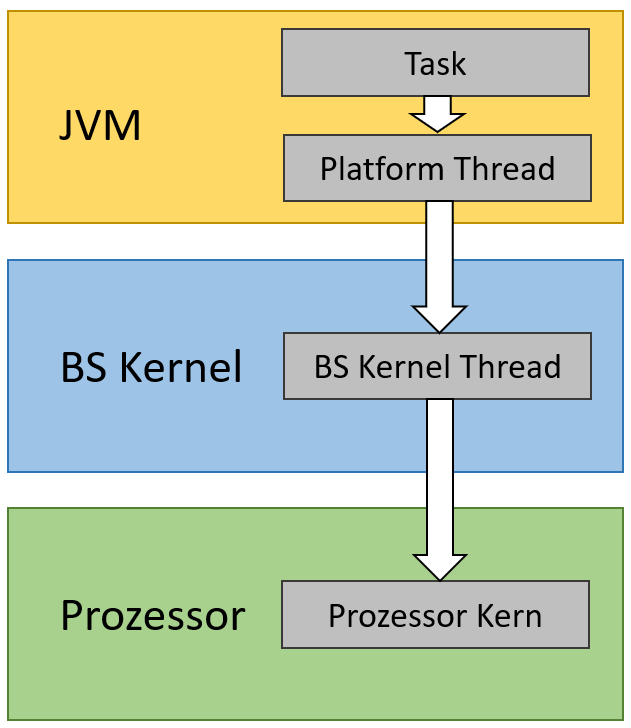
\includegraphics[scale=0.5]{figures/PlatformThreads.png}
	\caption{Aufbau: Java Platform Threads}
	\label{fig:PlatformThreads}
\end{figure}

Dieser Aufbau hat zur Folge, dass Plattform Threads schwergewichtig sind. Schwergewichtig mein in diesem Fall, das ein Plattform Thread viel Speicher verbraucht($\sim$ 2-3 MB) und es lange dauert ihn zu erstellen($\sim$ 1ms). Platform Threads und die dazugehörigen Betriebssystem Threads sind also ressourcenintensiv und ihre maximale Anzahl ist somit für ein ausführendes System begrenzt. Dies führt dazu, dass die maximale Anzahl der Platform Threads, weit vor anderen Ressourcen, zum limitierenden Faktor wird. 

Eine Lösung um zumindest die Kosten für das Erstellen von neuen Platform Threads zu senken, ist das Verwenden von Thread Pools. Hierbei wird eine Gruppe von Aufgaben einem Pool von Platform Threads zugewiesen. In der Regel übersteigt dabei die Anzahl der Aufgaben die Anzahl an Platform Thread. Dies hat zur Folge, dass einem Plattform Thread, nachdem er die ihm zugewiesene Aufgabe abgearbeitet hat, dierekt eine neue Aufgabe zugewiesen wird. Das hat den Vorteil, dass nicht mehr für jede Aufgabe ein neuer Platform Thread erstellt werden muss, statdessen können die gleichen Plattform Threads wiederverwendet werden um mehrere Aufgaben hintereinander auszuführen. Damit lassen sich zwar die Kosten für das Erstellen von neuen Platform Threads senken. Es lässt sich jedoch nicht die maximale Anzahl an Platform Threads erhöhen.

Ein weiteres Problem ist, dass die Verwaltung der Threads vom Betriebssystem über\-nommen wird und die JRE(Java Runtime Environment) keinen Einfluss darauf nehmen kann. Die Verwaltung der Threads auf Betriebssystemebene muss jedoch sehr allgemein gehalten werden, da sie nicht nur für Java, sondern für alle Programmiersprachen funktionieren muss.

\section{Java: Virtual Threads}

Java Virtual Threads waren erstmals im JDK 19(Java Development Kit) in Form einer Vorschauversion enthalten. Seit dem JDK 21 sind sie ein fester Bestandteil von Java. Sie wurden ursprünglich im Rahmen des Project Loom als sogenannte Fiebers entwickelt. Das Ziel war es die mittlerweile nicht mehr zeitgemäßen Java Threads, durch eine leichtgewichtigere Variante zu ersetzen, welche auf die gleiche API(Application Programming Interface) zurückgreift.

Das Ziel von Virtual Threads besteht in der Umgehung der Schwachstellen von Platform Threads, indem eine große Anzahl Virtual Threads auf eine kleine Zahl Betriebssystem Threads verteilt wird. Dadurch kann eine deutlich größere Anzahl an Virtual Threads gleichzeitig erstellt werden, welche von der JRE verwaltet werden.

Im Detail sieht dies wie folgt aus:

Es wird eine kleine Anzahl an Platform Threads(Wrapper) erstellt, die ihrerseits einen Betriebssystem Thread umschließen. Diese Platform Threads werden als Carrier Threads bezeichnet und ihre Anzahl entspricht standardmäßig der Anzahl der Prozessorkerne des ausführenden Systems, kann jedoch je nach Anwendungsfall leicht variieren. Die Carrier Threads werden von einem ForkJoinPool verwalten der nach dem FIFO-Prinzip(First In - First Out) und mit work-stealing arbeitet.\cite{Pressler2023a}

Für jede neue Aufgabe(task) im System, die nebenläufig ausgeführt werden kann, wird ein neuer Virtual Thread erstellt. Die Aufgabe bleibt dabei die ganze Zeit im gleichen Virtual Thread. Der Virtual Thread wiederum wird zum bearbeiten der Aufgabe in einen Carrier Thread eingesetzt(mount). 

\begin{figure}[h]
	\centering
	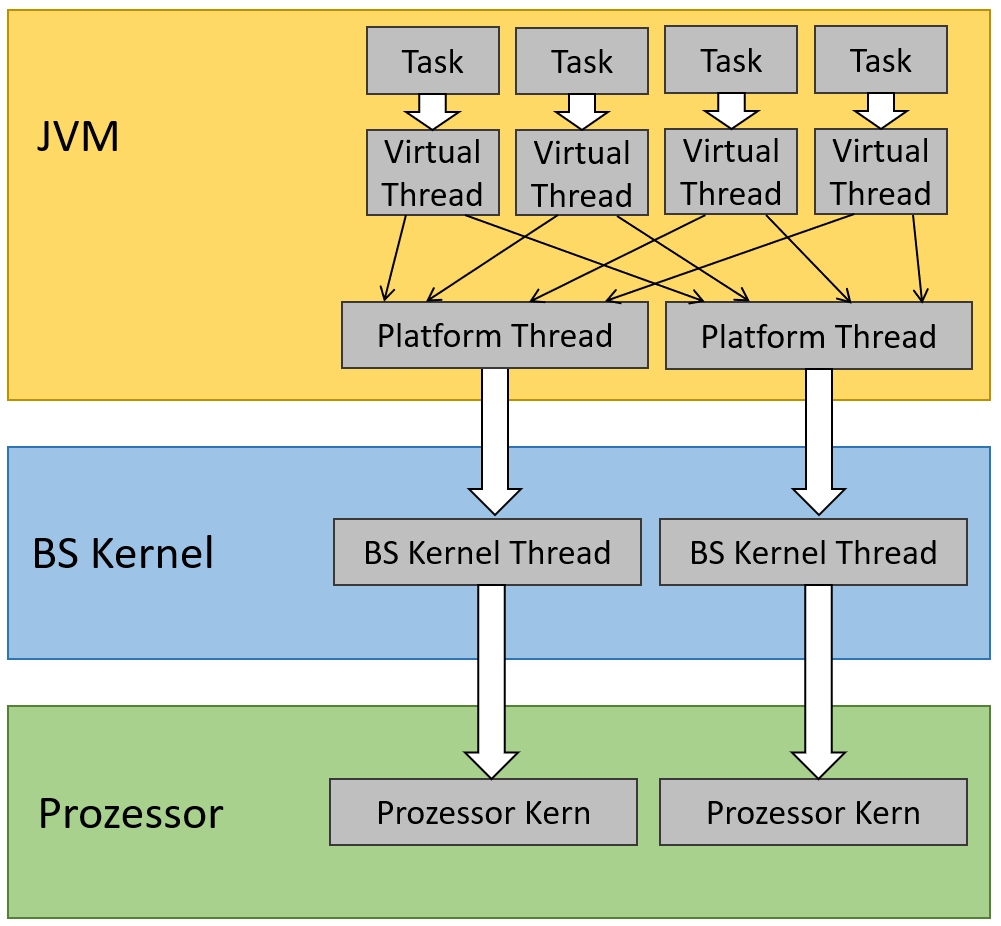
\includegraphics[scale=0.5]{figures/VirtualThreads.png}
	\caption{Aufbau: Java Virtual Threads}
	\label{fig:VirtualThreads}
\end{figure}


Dort bleibt der Virtual Thread so lange bis die Aufgabe abgeschlossen ist oder der Thread blockiert. Sollte es zu einer Blockade, zum Beispiel durch eine I/O-Operation, kommen, wird der Virtual Thread aus dem Carrier Thread entnommen(unmount) und so lange geparkt bis er nicht mehr blockiert ist und die Bearbeitung der Aufgabe fortgesetzt werden kann. Der Virtual Thread wir dann wieder in eine freien Carrier Thread eingesetzt, dies kann aber ein andere sein als zu Beginn. Daraus folgt, eine Aufgabe wird ihre gesamte Lebenszeit vom gleichen Virtual Thread ausgeführt, welcher jedoch in unterschiedliche Carrier Threads eingesetzt werden kann. Dies hat den Vorteil, dass ein Virtual Thread ein Betriebsystems Thread nur dann benutzt, wenn der Virtual Thread Berechnungen auf dem Prozessor ausführt. Ist ein Virtual Thread blockiert macht er platzt auf dem Betriebsystem Thread für einen anderen Virtual Thread. Dies führt zu einer effizienteren Auslastung des Prozessors.\cite{Bateman2023}

\begin{figure}[h]
	\centering
	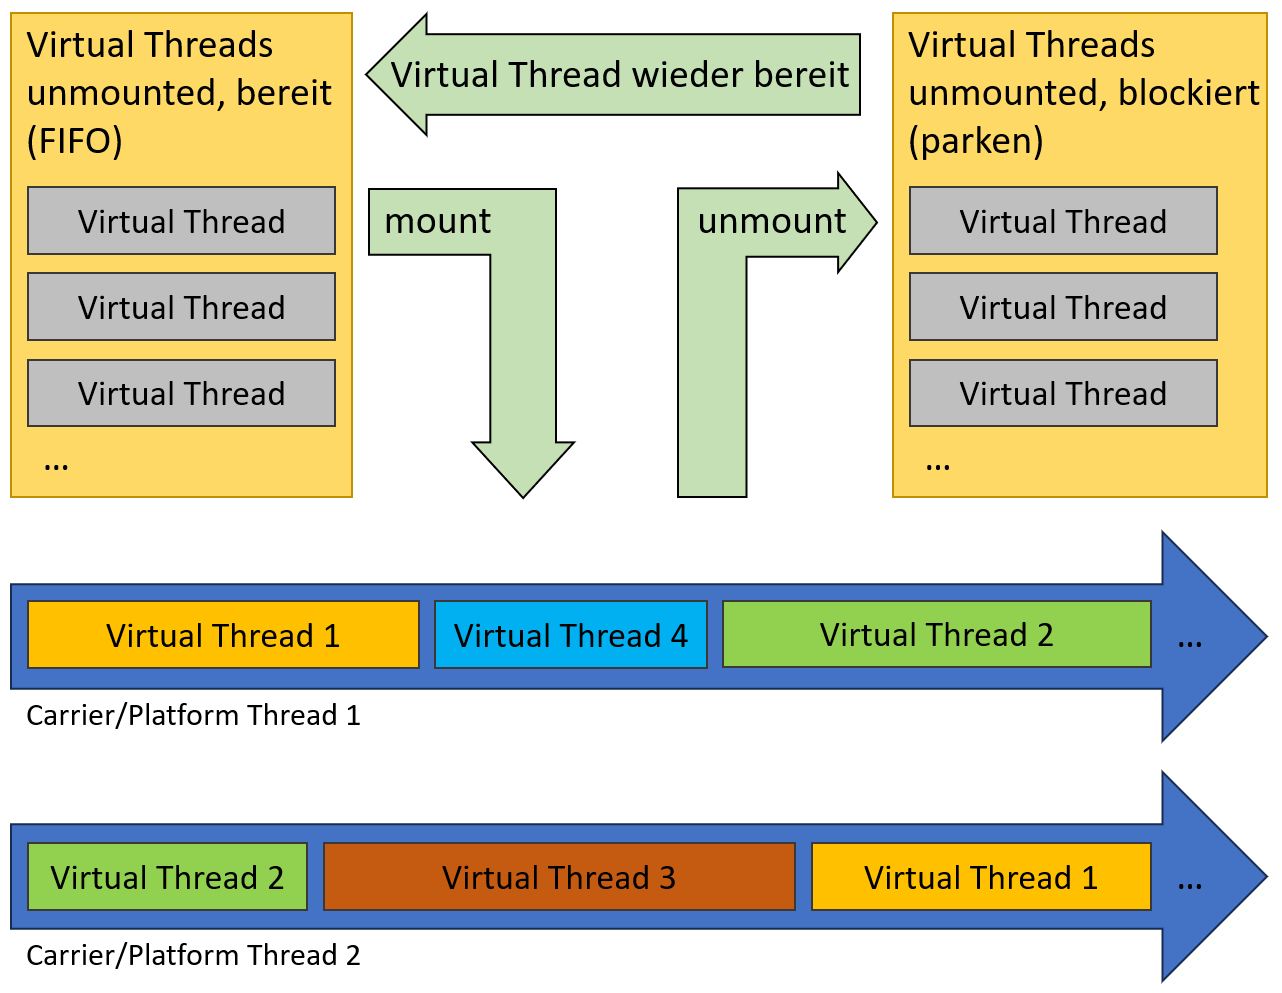
\includegraphics[scale=0.5]{figures/VirtualThreadsAblauf.png}
	\caption{Verwaltung: Java Virtual Threads}
	\label{fig:VirtualThreadsAblauf}
\end{figure}

\subsection{Continuations}

Das beschriebene Starten(mount) und Parken(unmount) von Virtual Threads wird mit Continuations gelöst. Ein Virtual Thread umschließt die ihm übergeben Aufgabe mit einer Continuation. Diese bietet die Methode \code{Continuation.run()} an, um enthaltene Aufgabe entweder zum ersten mal zu starten oder sie nach dem parken fortzusetzen. Letzteres wird auf der Ebene der Continuations als Auftauen(thaw) bezeichnet. Des weiteren gibt es die Methode \code{Continuation.yield()} um eine Aufgabe zu pausieren, wenn sie blockiert. Dies wird im Kontext der Continuations als einfrieren(freez) bezeichnet. Zu letzt stellen Continuations noch die Methode \code{Continuation.isDone()}(Rückgabewert: boolean) zur Verfühgung, um zu überprüfen ob die enthaltene Aufgabe abgeschlossen wurde. Um die Funktionalität der Continuations umzusetzen, musste das gesamte JDK auf Stellen überprüft werden, an denen eine Aufgabe potenziell blockieren kann. An entsprechenden Stellen musste neuer Code hinzugefügt werden, der mit den Continuations kommuniziert, um so eine Aufgabe entweder einzufrieren oder später wieder aufzutauen.\cite{Pressler2023b}

Wenn es um das Blockadeverhalten von Virtual Threads geht gibt es einen Spezialfall, der nach Möglichkeit vermieden sollte, das sogenannte Festecken(pinning). Dies beschreibt den Fall, wenn die im Virtual Thread enthaltene Aufgabe blockiert und der Virtual Thread nicht aus dem ausführenden Carrier Thread entnommen werden kann. Dies führt dazu, dass nicht nur der Virtual Thread sonder auch der Carrier Thread blockiert. Dies kann entweder dadurch ausgelöst werden, dass der Thread blockiert während er nativen Code aufruft oder der Thread blockiert, während er Code ausführt der sich in einem Synchronized Block befindet. Sollte der Code im Synchronized Block lange blockieren, kann es sinnvoll sein das Synchronized durch ein Reentrant Lock zu ersetzen. Die Beschränkung durch Synchronized, soll laut den Virtual Thread Entwicklern in einer zukünftigen Version aufgehoben werden. Die Beschränkung durch das Aufrufen von nativen Code wird jedoch bestehen bleiben.\cite{Bateman2024}

\subsection{Thread per request Model}

Ein typischer Anwendungsfall für Virtual Threads ist ein Server-Anwendung die Anfragen im Thread per request Model bearbeitet. Für jede neue Anfrage wird ein neuer Thread erstellt der diese Anfrage bearbeitet. So können mehrere Anfragen nebenläufig berarbeitet werden. Dies würde bei Platform Threads bedeuten, dass für jede neue Anfrage nicht nur ein neuer Platform Thread sondern auch ein neuer Betriebssystem Thread erstellt werden muss. Da die Anzahl an Betriebssystem Thread aber für ein System stark limitiert ist, in der Regel einige Tausend Stück, ist damit auch die Anzahl der nebenläufig zu bearbeitenden Anfragen limitiert. So werden Plarform Threads zum limitierenden Faktor des Systems. Virtual Threads hingegen sind deutlich leichtgewichtiger, da ihre Anzahl nicht an die zur Verfühgung stehenden Betriebssystem Threads gebunden ist. Dadurch lässt sich eine große Anzahl von ihnen erstellen, bis zu mehrere Millionen Stück.

Der Vorteil von Virtual Thread gegenüber Platform Threads bei dem Thread per request Model, lässt sich gut an Littels Gesetz zeigen. Es besagt, dass die sich gleichzeitig in Bearbeitung befindlichen Aufgaben(L) davon abhängig sind wie hoch der Durchsatz($\lambda$) und die Durchlautzeit (W) sind.\cite{Little_1961}

\begin{eqnarray}
	L = \lambda \cdot W \nonumber
\end{eqnarray}

Daraus folgt, das der Durchsatz sich aus den gleichzeitig in Bearbeitung befindlichen Aufgaben und der Durchlaufzeit ergibt.

\begin{eqnarray}
	\lambda = \frac{L}{W} \nonumber
\end{eqnarray}

Auf das Thread per request Model angewandt, bedeutet das, dass der Durchsatz die pro Sekunde in das System eingehend Anfragen ist. Die Durchlaufzeit wird dadurch beschrieben wie hoch die durchschnittlich Latenz des Systems ist um eine Anfrage zu beantworten. 

Gehen wir also von einem System aus, das 200 Anfragen pro Sekunde verarbeitet, bei einer Latenz von 50ms pro Anfrage. Dafür ist es nötig 10 Anfragen gleichzeitig nebenläufig zu verarbeiten. Soll das System nun auf 2000 Anfragen pro Sekunde, bei gleichbleibender Latenz, skaliert werden, muss das System nun 100  Aufgeben gleichzeitig nebenläufig verarbeiten.

Da wir vom Thread per request Model ausgehen, müssen also im Fall von  Platform Threads, 100 von ihnen erstellt werden und damit auch 100 Betriebssystem Threads. Somit ist die Skalierbarkeit auf die maximal zur Verfühgung stehenden Betriebssystem Threads(einige Tausend) begrenzt. Virtual Threads hingegen lassen sich in einer deutlich größeren Anzahl erstellen(mehrere Millionen) und werden so nicht zum limitierenden Faktor wenn es um die Skalierbarkeit des beschriebenen Beispiels geht.

Die Annahme stimmt allerdings nur so lange, wie die nebenläufig bearbeiteten Aufgaben, weiterhin mit der gleichen Latenz bearbeitet werden. Dies ist zum Beispiel dann der Fall, wenn ein Aufgabe pausiert wird um auf I/O-Operation zu warten. Wenn die einzelne Aufgaben jedoch rechenintensiv sind und möglicherweise niemals pausieren verlieren Virtual Threads ihren Vorteil gegen über Platform Threads. Virtual Threads können nicht einzelne Aufgaben schneller ausführen als Platform Threads, sondern mehr Aufgaben nebenläufig bearbeiten. Damit lässt sich abschließend sagen Virtual Threads steigern den Durchsatz einer Anwendung gegenüber Platform Threads, wenn viele Aufgaben nebenläufig ausgeführt werden und die Rechenlast der einzelnen Aufgaben niedrig ist.

\subsection{Softwareentwicklung mit Virtual Threads}

Eine weitere Zielsetzung von Virtual Threads war es Softwareentwicklern den umstieg von Plattform Threads zu Virtual Threads so einfach wie möglich zu gestalten. Deshalb sind Virtual Threads genau wie Plattform Threads eine Instanz der \code{java.lang.Thread} API. So ist es relativ einfach möglich Virtual Threads zu integrieren ohne die bestehende Codebasis wesendlich zu verändern.

Am folgendem Code-Beispiel wird deutlich, es muss lediglich der Aufruf \code{Thread.ofPlatform()} durch \code{Thread.ofVirtual()} ersetzt werden, der restliche Code bleibt unberührt.

\begin{lstlisting}[language=Java]
	//erstellen eines einzelnen Platform Threads
	Thread platformThread = Thread.ofPlatform().start(() -> System.out.println("Platform Thread"));
	platformThread.join();

	//erstellen eines einzelnen Virtual Threads
	Thread virtualThread = Thread.ofVirtual().start(() -> System.out.println("Virtual Thread"));
	virtualThread.join();
\end{lstlisting}

Für Virtual Threads wurde der neue Executor Service \code{Executors.newVirtualThreadPerTaskExecutor()} entwickelt. Für jeden Aufruf von \code{ExecutorService.submit(Runnable)} wird ein neuer Virtual Thread erstellt, der die ihm zugewiesene Aufgabe ausführt. Der Rückgabewert des Executor Service ist ein Future, welches das Ergebnis der Aufgabe enthält so bald der erstellte Virtual Thread ausgeführt wurde. Mit Hilfe von \code{Executors.newVirtualThreadPerTaskExecutor()} lässt sich bestehender Code leicht von Platform Threads auf Virtual Threads umstellen. Oft wird für das Verwalten von Platform Threads ein Thread Pool erstellt und für das Erstellen eines Thread Pools ein Executor Service verwendet. So könnten die Plattform Threads beispielsweise bisher in \code{Executors.newCachedThreadPool()} verwaltet worden sein. Dieser lässt sich nun leicht durch \code{Executors.newVirtualThreadPerTaskExecutor()} ersetzen. Dies wird auch am folgenden Beispiel deutlich:

\begin{lstlisting}[language=Java]
	//mehrere Platform Threads mit Executors.newCachedThreadPool() erstellen
	try (var cachedPool = Executors.newCachedThreadPool()) {
		var future1 = cachedPool.submit(() -> powerFunction(task1.base, task1.exponent));
		var future2 = cachedPool.submit(() -> powerFunction(task2.base, task2.exponent));
		int ptResult1 = future1.get();
		int ptResult2 = future2.get();
	
		System.out.println("Platform Thread Result 1: " + ptResult1);
		System.out.println("Platform Thread Result 2: " + ptResult2);
	} catch (ExecutionException | InterruptedException e) {
		throw new RuntimeException(e);
	}

	//mehrere Virtual Threads mit Executors.newVirtualThreadPerTaskExecutor() erstellen
	try (var executor = Executors.newVirtualThreadPerTaskExecutor()) {
		var future1 = executor.submit(() -> powerFunction(task1.base, task1.exponent));
		var future2 = executor.submit(() -> powerFunction(task2.base, task2.exponent));
		int vtResult1 = future1.get();
		int vtResult2 = future2.get();
	
		System.out.println("Virtual Thread Result 1: " + vtResult1);
		System.out.println("Virtual Thread Result 2: " + vtResult2);
	} catch (ExecutionException | InterruptedException e) {
		throw new RuntimeException(e);
	}
\end{lstlisting}

Dabei wird deutlich das für Virtual Threads kein Thread Pool benötigt wird. Ihre maximal Anzahl ist deutlich größer als die von Platform Threads und die Zeit sie zu erstellen und ihr Speicherverbrauch sind deutlich geringer. Daher sollten Virtual Thread niemals in einem Thread Pool verwaltet werden. Bei der Umstellung auf Virtual Threads werden Platform Threads also nicht direkt durch Virtual Threads ersetzt. Stattdessen werden die Aufgaben durch Virtual Threads ersetzt, beziehungsweise für jede Aufgabe wird ein neuer Virtual Thread erstellt. Falls ein Thread Pool bei Platform Threads bisher verwendet wurde um die Anzahl an maximal nebenläufig ausgeführten Aufgaben zu limitieren, sollte dafür bei Virtual Threads sattdessen auf Semaphore zurückgegriffen werden.

\newpage

\section{Kotlin: Coroutinen}

Coroutinen sind ein zentrales Konzept in Kotlin, das für asynchrone Programmierung und nebenläufige Prozesse verwendet wird. Coroutinen sind eine Art von leichtgewichtigen Threads, mit denen es möglich ist Funktionen anzuhalten und später wieder fortzusetzen. Dies erlaubt es, komplexe asynchrone Programmabläufe einfacher zu schreiben und leichter zu verstehen. Dieses Kapitel wird die Grundlagen von Coroutinen, deren Implementierung und fortgeschrittene Anwendungsfälle erklären.

\subsection{Motivation}

Bevor es Coroutinen in Kotlin gab, wurde asynchroner Code häufig mit Callbacks umgesetzt. Dabei handelt es sich um ein Programmierkonzept bei dem einer Funktion als Argument eine anderen Funktion übergeben wird, um zu einem späteren Zeitpunkt aufgerufen zu werden. Dies ermöglicht eine flexible und modulare Struktur von Programmen, da verschiedene Operationen oder Ereignisse mit spezifischen Reaktionen verknüpft werden können. Callbacks sind besonders nützlich in der asynchronen Programmierung, wo Operationen wie das Lesen von Dateien, das Abrufen von Daten über das Netzwerk oder das Warten auf Benutzereingaben ohne Blockieren des Hauptprogramms ausgeführt werden können. 

\begin{lstlisting}[language=Kotlin]
	import java.io.File
	import kotlin.concurrent.thread
	
	fun readFileAsync(filename: String, callback: (String) -> Unit) {
		thread {
			val content = File(filename).readText()
			callback(content)
		}
	}
	
	fun main() {
		readFileAsync("example.txt") { content ->
			println("File Content: $content")
		}
		println("Read File...")
	}
\end{lstlisting}

In dem gezeigten Beispiel liest die Funktion \code{readFileAsync} den Inhalt einer Datei in einem separaten Thread ein und verwendet einen Callback, um das Ergebnis zurückzugeben. Der Callback wird als Lambda-Ausdruck an \code{readFileAsync} übergeben und ausgeführt, nachdem das Einlesen abgeschlossen ist. Der Haupt-Thread wird währenddessen nicht blockiert und kann andere Aufgaben ausführen.

Ein Nachteil von Callbacks ist jedoch die Verwendung vieler verschachtelter Callbacks, welche umgangsprachlich als Calback Hell bezeichnet werden. Sie führt dazu das der Code schwer lesbar wird. Was wiederum zu einer erhörten Komplexität bei der Wartbarkeit und dem Debudden führt, da die Rückverfolgung des Programmflusses kompliziert wird. Außerdem wird die Fehlerbehandlung immer aufwendiger, da sie auf jeder Ebene der Verschachtlung stattfinden muss.

\begin{lstlisting}[language=Kotlin]
	fun firstOperation(callback: (String) -> Unit) {
		// Simulierte asynchrone Operation
		callback("Result 1")
	}
	
	fun secondOperation(input: String, callback: (String) -> Unit) {
		// Simulierte asynchrone Operation
		callback("$input -> Result 2")
	}
	
	fun thirdOperation(input: String, callback: (String) -> Unit) {
		// Simulierte asynchrone Operation
		callback("$input -> Result 3")
	}
	
	fun main() {
		firstOperation { result1 ->
			secondOperation(result1) { result2 ->
				thirdOperation(result2) { result3 ->
					println("Final Result: $result3")
				}
			}
		}
	}
\end{lstlisting}

In diesem Beispiel werden drei Operationen asynchron mit Callbacks ausgeführt, die jeweils das Ergebnis der vorausgehenden Operation benötigen. Dies führt zu einer Verschachtlung der Aufrufe in der Main-Funktion. Selbst in diesem einfachen Bespiele wird der Code schon deutlich schwerer lesbar im Vergleich zu einer synchronen Programmierweise. Obwohl sogar in diesem Beispiel auf Fehlerbehandelung verzichtet wurde.

Genau an diesem Punkt setzte die Entwicklung von Coroutinen an, welche als Ziel hatten die Nachteile der Callback Hell zu umgehen und dabei trotzdem die Vorteile der Callbacks zu behalten.


\subsection{suspend-Modifier}

Um die Nachteile der Callback Hell zu umgehen, verfolgen die Coroutinen den Ansatz, das synchroner Code geschrieben wird, welcher dann asynchron ausgeführt wird. Dafür wurde der Modifier suspend eingeführt. Dadurch kann das Code-Beispiel aus dem vorausgehenden Kapitel folgender maßen optimiert werden:

\begin{lstlisting}[language=Kotlin]
	import kotlinx.coroutines.*
	
	suspend fun firstOperation(): String {
		// Simulierte asynchrone Operation
		return "Result 1"
	}
	
	suspend fun secondOperation(input: String): String {
		// Simulierte asynchrone Operation
		return "$input -> Result 2"
	}
	
	suspend fun thirdOperation(input: String): String {
		// Simulierte asynchrone Operation
		return "$input -> Result 3"
	}
	
	fun main() = runBlocking {
		val result1 = firstOperation()
		val result2 = secondOperation(result1)
		val result3 = thirdOperation(result2)
		println("Final Result: $result3")
	}
\end{lstlisting}

In dem Beispiel werden jene Funktionen mit dem suspend-Modifier gekennzeichnet, die als asynchrone Operationen ausgeführt werden solle. Die Funktion runBlocking startet eine Coroutine und blockiert den aktuellen Thread bis die Coroutine beendet ist. Die Coroutine wiederum führt die drei suspend Funktionen aus.

Dadurch ist es möglich in der Main-Funktion eine synchrone Schreibweise zu verwenden, was die Lesbarkeit gegenüber dem Callback-Ansatz deutlich erhöht. Generell ist bei der Verwendung von supend-Funktionen zu beachten, dass sie nur von anderen suspend-Funktionen oder Coroutinen ausgeführt werden können.

\subsection{Coroutinen starten}

Um in Kotlin eine Coroutine zu starten wird ein Coroutinen-Builder verwendet. Dies sind die am häufigsten verwendeten Coroutinen-Builder:

\subsubsection{launch}

lauch ist der am häufigsten verwendete Coroutine-Builder und startet eine neue Coroutine, die kein Ergebnis zurückgibt. Er wird hauptsächlich für nebenläufig auszuführende Aufgaben verwendet, die nach dem fire-and-forget Prinzip gestartet werden.

\subsubsection{async}

async startet ebenfalls eine neue Coroutine, gibt aber ein Deferred-Objekt zurück, das ein zukünftiges Ergebnis repräsentiert. Bei Deferred handelt sich um das Äquivalent eines Promis oder Future in Kotlin. Mit ist es möglich auf das Ergebnis zu warten.

\subsubsection{runBlocking}

runBlocking blockiert den aktuellen Thread, bis der Coroutine-Block abgeschlossen ist. Es wird hauptsächlich in Main-Funktionen und Testfällen verwendet.

\subsubsection{produce}

produce ist ein spezieller Coroutine-Builder, der eine ReceiveChannel erstellt und Werte in diesen Kanal sendet. Es wird hauptsächlich für Producer-Consumer-Muster verwendet.

\subsubsection{run}

run ist ein allgemeiner Coroutine-Builder, der eine Coroutine startet und das Ergebnis des letzten Ausdrucks im Block zurückgibt.


\subsubsection{Coroutinen-Builder}

Das folgende Beispiel zeigt den aufbau eines Coroutinen-Builders, anhand der Funktionssignatur des Builders launch.

\begin{lstlisting}[language=Kotlin]
fun CoroutineScope.launch(
context: CoroutineContext = EmptyCoroutineContext,
start: CoroutineStart = CoroutineStart.DEFAULT,
block: suspend CoroutineScope.() -> Unit
): Job
\end{lstlisting}

Die Funktionssignatur besteht aus dem Empfänger-Typ CoroutineScope, Funktionsnamen launch, den Parametern context, start, block und dem Rückgabewert Job.

TODO: Verweis auf spätere Kapitel

Der start Parameter gibt an, wann die Coroutine gestartet wird. Dafür kann eine CoroutineStart Enumeration übergeben werden. Der Standardwert ist CoroutineStart.DEFAULT, was bewirkt, dass die Coroutine sofort gestartet wird.

TODO: block erklären 

\subsection{Job}

Ein Job Objekt in Kotlin repräsentiert eine Coroutine und ihreren Lebenszyklus. Ein Job wird dafür verwendet, um den Status einer Coroutine zu überwachen und zu kontrollieren. Der Coroutinen-Builder launch hat zum Beispiel ein Job Objekt als Rückgabewert für genau diesen Zweck. Um den Status der Coroutine zu überwachen stehen folgende Eigenschaften zur Verfügung:

\begin{itemize}
	\item isActive: Gibt true zurück, wenn der Job aktiv und nicht abgeschlossen oder abgebrochen ist.
	\item isCompleted: Gibt true zurück, wenn der Job abgeschlossen ist.
	\item isCancelled: Gibt true zurück, wenn der Job abgebrochen wurde.
\end{itemize}

Um eine Coroutine zu kontrollieren stellt ein Job folgende Methoden zur Verfügung:

\begin{itemize}
	\item start(): Startet den Job, falls er noch nicht gestartet wurde.
	\item cancel(): Bricht den Job ab. Alle untergeordneten Coroutinen werden ebenfalls abgebrochen.
	\item join(): Eine suspendierende Funktion, die wartet, bis der Job abgeschlossen ist.
	\item invokeOnCompletion(handler: CompletionHandler): Fügt einen Handler hinzu, der ausgeführt wird, wenn der Job abgeschlossen ist.
\end{itemize}

TODO: Hierarchische Beziehungen Verweis

Auch das Deferred Objekt ist ein Job Objekt. Es wird beispielsweise von dem async Coroutinen-Builder zurückgeben. Es hat neben den oben genannten Eigenschaften und Methoden, noch folgende weiter Methoden um die Funktionalität eines Futures erfüllen zu können:

\begin{itemize}
	\item await(): Eine suspendierende Funktion, die auf das Ergebnis der Coroutine wartet und es zurückgibt.
	\item getCompleted(): Gibt das Ergebnis zurück, wenn die Coroutine abgeschlossen ist, oder wirft eine Ausnahme, wenn die Coroutine noch nicht abgeschlossen ist oder mit einem Fehler beendet wurde.
\end{itemize}



\subsection{Stichpunkte}

coro starten mit builder
hat rückgabe wert zB future
optionaler übergabewert: context
invoker weiss dann welcher executioncontext genutzt wird



Context: auf welchem Thread soll Code Laufen?
Dispatcher?
-Main: optimiert fur UI/ non-blocking Code (kurze laufzeit)
-IO: optimiert für Netzwerk oder Disk operationen
-Default: CPU-intensive / große Berechnungen

Coro laufen auf Threads
können suspended werden
-pausiert, aus Thread entfernt, in SPeicher gelegt
-Thread wieder frei

Coro Scope?
jede Coro muss in einen Scope ausgeführt werden
-1 GlobaleScope: für TopLevel Coro, lebt so lange wie die ANwendung, Risiko Memory leaks
-2 lifeCicleScope:verknüpft mit lifecycle von Fragment oder activity, wen Frag zerstört onDestroy()
-3 ViewModleScop: lifeCycle of viewModel, onClear()

2,3: automatische Cancellation, keine memory leaks, räumt hinter sich auf

Beispiel:
val scope = CoroutineScope(CoroutineName("myScope"))
Scope.launch{
	this.coroutineContext.toString()
}
Ausgabe: Name, Job, Dispatcher

CoroScope(CoroContext)
CoroContext = Job + Dispatcher +CoroName
Beispiel: wenn Coro 2 im Scope von Coro1 gestartet wird
dann -erbt Context -Job2 Kind von Job1 (vererbung)
wenn Coro1 abgebrochen dan Coro2 abgebrochen
Vererbung VOrteil leichter aufräumen da wenn elter abgebrochen auch kinder

Job?
-Coro lifecycle
-Cacellation
-Parent-child relations

mehere Coro in einem Scope ausfürhren
wenn Scope canceled alle (child)Cror canceled

delay()? -> sleep?
yield()?
suspend fun aus kotlinx

kotlinx?

JobStates:
-isActive
-isCompleted
-isCancelled

cooperative? -> make canclebel
-isActive
-ensureActive
-uspend fun aus kotlinx

Chanelles
Mehrere Producer möglich
Mehrere Reciver möglich
Daten bleiben in Reihenfolge
TODO: Bild Channel

Channel Types:
Buffered: Max Capacity festlegen, suspend bis Platz
Conflated: MaxCap = 1, neu Elemente ersetzen alte
Rendezvou: Default, Buffered, MaxCap = 0, wird nur gesendet wenn es Empfänger gibt
Unlimited: Buffered, unbegrenzte Buffered Capa, Risiko für outOfMemoryEx.

Futures/Promises/Rx, Problem viele Combinators
für jede Futur bibliothek unterschiedliche Combinators


Countinuation Passing Style(CPS)
eigentlich Callbacks, zu viele Verschachtelungen

Direct Style: Code bleibt gleich -> Coroutinen unterstützen das

CPS Transformation(passiert im Compiler, also Byte Code-Ebene)
von:
Kotlin, direct Style, suspedn function

zu:
Java/JVM, CPS, Continuation(Callback)

Continuations is generic callback interface
Aufzählung Methoden?!

1. State: object(Aktueller Stand)->State Machine(ist eine Continuation)
	enthält lable, Rückgabewerte
2. Label: was als nächstes, Suspend Punkte im Code markiert?!
...?!

State Machine:
wiederverweten von closure und stateobject
einfach für loops

vs.

Callbacks:
für jede Verschachtelung neues Closure
loops sehr schwer umzusetzen?! warum?

call with current continuation kommt aus Scheme (WIkipedia?!)
suspend Coroutine
suspend fun (reguläre Function)

Coroutine Context
interface Continution Intercepter
auf welchem Thread soll ausgeführt werden

Dispatcher(bei invoke oder resume)
dispatches execution to another thread
normalerweise UI oder Thread Pool


job canncellaiton
launch builder gibt job object zurück
kann coro manipulieren
job.join()
job.cancel()

cooperative cancellation
muss abbrechbar sein an erwartbaren pubkten

code beispiel 
while true/isActive nicht/ist
spending fun aus öibrary alle caneble zB delay()

Communicating sequentail Process (CSP)
named Channels / prozesse annonyme
viele prozesse die nebenläufig sind, prozesse im inneren sequentiel

kein shared mutable state

actors
actor= named coro + inbox chanel
es wir dierect an actor statt an chanell gesendet

beides gut für skalierbarkeit


\section{Kotlin: Threads}

\section{Go: Go-Routinen}

\section{C\#: async/await}

\section{Vergleich der Konzepte}



\chapter{Benchmarks}

\section{Benchmark 1}

\section{Benchmark 2}

\section{Benchmark 3}

\section{Benchmark 4}



\chapter{Testaufbau}

\section{Testumgebung}

\section{Performancefaktoren}

\section{Werkzeuge zur Datenerhebung}
jcmd
jfr



\chapter{Messungen}

\section{Messung: Benchmark 1}

\section{Messung: Benchmark 2}

\section{Messung: Benchmark 3}

\section{Messung: Benchmark 4}



\chapter{Auswertung}

\section{Ergebnisse und Beobachtungen}

\section{Diskussion und Bewertung}



\chapter{Zusammenfassung und Ausblick}

\section{Zusammenfassung}

\section{Ausblick}
Java VT kein pinning bei Synchronized
Structured Concurrency(jeps/preview)
Scoped Values(jeps/preview)

\printbibliography


%\input{abkuerz.tex}      % Einbinden von Tex-Files
%\input{einfuehrung.tex}
%
%\include{normen}        % Einbinden von größeren Tex-Files,z.B. Kapiteln
%\include{aufbau}
%\include{zitieren}
%\include{form}
%\include{allgtips}
%
%\bibliographystyle{alpha}  % Schlüssel als Buchstaben
%\bibliography{literaturverzeichnis}      % Literaturverzeichnis

\end{document}


